\mysubsection{Interface Homme $ \leftrightarrow $ Machine}

L'objectif de cette structure de travail a été concevoir une interface graphique entre l'utilisateur et l'ordinateur qui permet à deux joueurs de réaliser séquentiellement leurs mouvements que puissent être réalisés par le robot sur un tableau réel. En prenant en compte cet objectif et les limitations pour l'exécution de ces tâches, on a construit une interface fonctionnelle, intuitive et déployée de façon plus simple. Alors, on a choisi de développer l'interface par programmation en langage Matlab et de manière modularisée, à savoir, la séparation des différentes tâches en différentes fonctions et avec un haut niveau d'indépendance.
\vspace{3pt}
\begin{figure}[H]
	\begin{center}	
		\captionsetup{justification=centering,margin=1cm}
		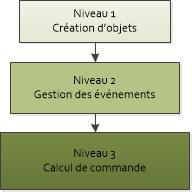
\includegraphics[width=8cm]{./diagrama_nivel.jpg}
		\caption{Les trois différentes niveaux des fonctions de construction de l’IHM}
		\label{fig:diagrama_nivel}
	\end{center}
\end{figure}

Les fonctions du niveau 1 sont concernant l'insertion et réglage des éléments graphiques dans l’interface. Ainsi, au début on a besoin de définir les variables du jeu que doivent être paramétrés et reçus par l’interface et ensuite on a pu mettre les objets graphiques dans l’interface et faire le réglage. 
 
Les fonctions du niveau 2 sont concernant la gestion des événements générés en chaque objet de l’interface. Ainsi, ces fonctions sont responsables d’appeler les fonctions d'intégration avec les algorithmes de calcul de trajectoire et commande, en plus de gérer la structure de données et mettre à jour les paramètres d’entrée des différentes fonctions d’interface.
 
Les fonctions du niveau 3 sont composées par les fonctions qui intègrent le calcul de trajectoire et le module de commande. Ainsi, elles calculent les trajectoires et couples nécessaires pour le robot réaliser les différentes mouvementés générés sur l’interface graphique.
\pagebreak

\begin{figure}[H]
	\begin{center}
		\captionsetup{justification=centering,margin=1cm}	
		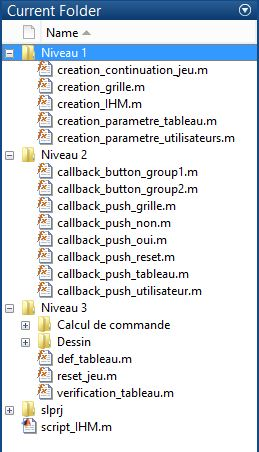
\includegraphics[width=5cm]{./current_folder.JPG}
		\caption{Le dossier des fonctions de l’IHM}
		\label{fig:folder}
	\end{center}
\end{figure}

